\chapter{The Friedmann equation and the thermal history of the universe}

In this chapter we continue with the discussion of the Friedmann equation that we started in the previous chapter. In particular, we will see how the presence of dark energy dramatically affects the evolution of the universe at late times. We will then begin the study of the thermal history of the universe. At early times, the particles in the universe form a fluid in thermodynamic equilibrium with a well-defined temperature. This temperature decreases as the universe expands, with the consequence that the properties of this cosmic fluid change in time (hence the name ``thermal history''), and in particular, some particle species decouple from the fluid at certain stages. One of the most important stages is the one in which the photons of the cosmic fluid decouple (when the universe was around $380,000$ years old) and begin to travel freely with no further interactions with other particles. These are the photons that we can observe today in the cosmic microwave background (CMB).

\section{The Friedmann equation (continued)}

\subsection{The FRW metric: summary}

We begin with a summary of the Friedmann-Robertson-Walker (FRW) metric. Recall that the cosmological principle, that is, the experimental fact that the universe is homogeneous and isotropic on large scales, implies that the universe must be described mathematically by the metric
\begin{equation} \label{eq:frw_metric}
ds^2=-c^2dt^2+a(t)^2\left[\frac{dr^2}{\left(1-k\frac{r^2}{R^2}\right)}+r^2\left(d\theta^2+\sin^2\theta d\phi^2\right)\right].
\end{equation}
This is known as the FRW metric. Actually, depending on the value of the parameter $k$, the expression in (\ref{eq:frw_metric}) describes three different spacetimes. For $k=0$ the spacetime has zero spatial curvature,\footnote{By spatial curvature we mean the curvature of the 3-dimensional spaces whose geometry is described by eq.\ (\ref{eq:frw_metric}) with $t=\mathrm{constant}$. In mathematical language, these spaces are called the spatial slices of the spacetime (\ref{eq:frw_metric}).} which implies that two light rays that start traveling parallel to each other will remain parallel. For $k=1$ the spacetime has positive spatial curvature, implying that two light rays that start parallel will eventually converge. Finally, for $k=-1$ the spacetime has negative spatial curvature, and so two light rays that start parallel will eventually diverge. In the cases $k=1$ and $k=-1$, the ``amount'' of curvature is quantified by the {\it curvature radius} $R$; the larger $R$, the less curved the space is. The 
cosmological principle does not tell us what are the values of $k$ and $R$, so they need to be experimentally measured.

The function $a(t)$ is known as the {\it scale factor}.\footnote{The scale factor was introduced in chapter 4, section 4.3.} Recall from chapter 4 that, in any space, the distance between two infinitesimally close points is given by $ds$; if the points are separated by a finite distance then we would simply integrate $ds$. In spacetimes, on the other hand, where we also deal with a time dimension, the distance between two infinitesimally close points (or events) is also given by the spacetime interval $ds$, but with the important condition that the two points must have equal times (that is, the events must be simultaneous); otherwise $ds$ cannot be interpreted as a distance in the usual sense (recall that $ds^2$ does not even need to be positive). For example, in the case of an FRW spacetime the distance $dl$ between two simultaneous events would be given by eq.\ (\ref{eq:frw_metric}) with $t$ constant:
\begin{equation} \label{eq:frw_dist}
dl(t)=a(t)\left[\frac{dr^2}{\left(1-k\frac{r^2}{R^2}\right)}+r^2\left(d\theta^2+\sin^2\theta d\phi^2\right)\right]^{1/2}.
\end{equation}
The important thing to note here is that the distance $dl$ is a function of time because of the presence of the scale factor $a(t)$. The coordinates $(r,\theta,\phi)$ are comoving spherical coordinates.\footnote{Spherical coordinates were introduced in chapter 3, section 3.3.} The name ``comoving'' means that galaxies remain with the same coordinates $(r,\theta,\phi)$ as the universe expands.\footnote{This is an approximation that is valid on large scales. Remember that galaxies have a peculiar motion in addition to the motion due to Hubble's law (see chapter 4), which implies that the coordinates $(r,\theta,\phi)$ for a given galaxy will slightly change in time. This is negligible on large scales, however.} We can think of the grid defined by the coordinates $(r,\theta,\phi)$ to be expanding in time; galaxies have fixed positions on this grid, and therefore fixed values of $(r,\theta,\phi)$. The distances between galaxies, however, are not fixed in time; this is because distances do not only depend on the 
coordinates of the comoving grid, but also on the scale factor $a(t)$, as it is clear from eq.\ (\ref{eq:frw_dist}). Fig.\ \ref{fig:lec6_1} shows two galaxies on the comoving grid (with the coordinate $\theta$ omitted) at two different times; notice that, even though the comoving coordinates of each galaxy remain fixed, the distance between the two increases in time.
\begin{figure}[ht]
\begin{center}
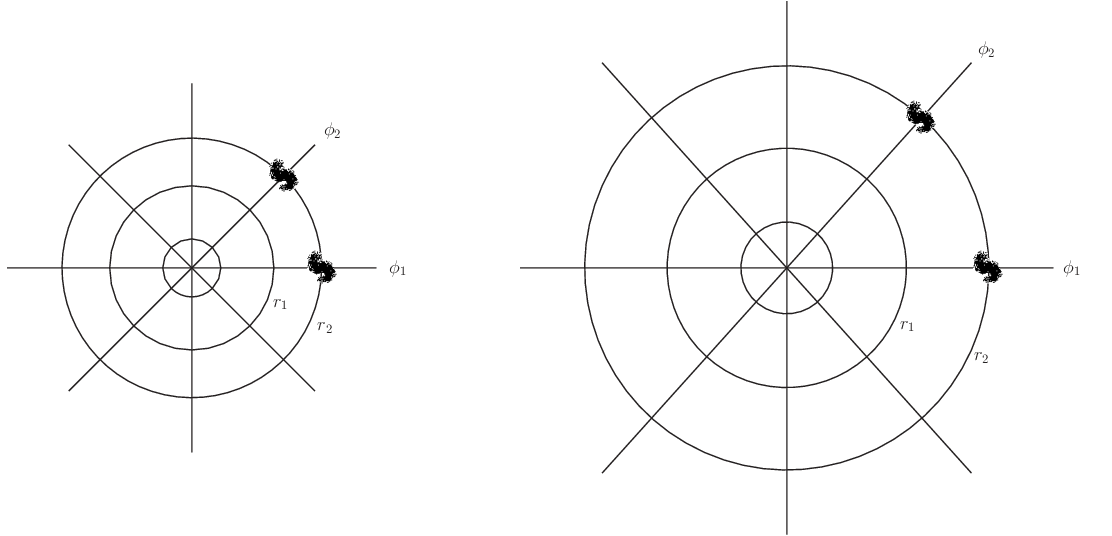
\includegraphics[scale=0.5]{Draw/lec6_1.png}
\end{center}
\caption{Comoving coordinates in the FRW metric}
\label{fig:lec6_1}
\end{figure}

\subsection{The Friedmann equation and the energy content of the universe}

We have learned that distances between objects in a homogeneous and isotropic universe change in time according to the scale factor, and therefore the function $a(t)$ is a direct measure of the expansion of the universe. The next step is to find how $a(t)$ changes in time, for which we need to make use of the Einstein equations. Recall that there are two ingredients in the Einstein equations: the metric (from which the Einstein tensor is constructed) and the energy-momentum tensor. We already have the metric, or more specifically, we have the form of the metric, since we do not know $a(t)$. We also know what is the form of the energy-momentum tensor: on large scales the matter in the universe can be well approximated as a perfect fluid.\footnote{The Einstein equations, the energy-momentum tensor, and perfect fluids were introduced in chapter 4.} With these ingredients the Einstein equations reduce to a simple differential equation that relates the scale factor $a(t)$ to the energy density $\rho(t)$:\footnote{
Notice that in chapter 5 we defined $\rho(t)$ as the {\it mass density} of the fluid, whereas here we adopt the more usual convention of defining $\rho(t)$ as the {\it energy density}. The only difference between the two is a factor of $c^2$.}
\begin{equation} \label{eq:friedmann_eq}
\left(\frac{\dot{a}}{a}\right)^2= \frac{8\pi G}{3c^2}\rho(t)-\frac{kc^2}{R^2a^2}.
\end{equation}
This is known as the {\it Friedmann equation}. We have adopted the notation
\begin{equation}
\dot{a}(t)\equiv \frac{da(t)}{dt}.
\end{equation}
Notice that we have made the assumption that the energy density depends only on time, not on position. This is a consequence of the cosmological principle: since all points in space are equivalent, they all must have the same energy density at any given time. In eq.\ (\ref{eq:friedmann_eq}) $\rho(t)$ denotes the {\it total} energy density, that is, the sum of the energy densities of all the sources present in the universe. There are three main types of sources: matter (with energy density $\rho_m(t)$), radiation (energy density $\rho_r(t)$), and dark energy (energy density $\rho_{\Lambda}$). Thus we can write
\begin{equation}
\rho(t)=\rho_m(t)+\rho_r(t)+\rho_{\Lambda}.
\end{equation}
Notice that the dark energy density $\rho_{\Lambda}$ is independent of time. The nature of dark energy is unknown, but one explanation is that it is an energy contained in the vacuum. Since the vacuum does not care about the expansion of the universe (which is a gravitational effect), the density of dark energy is thought to be constant in time.\footnote{We will say a lot more about dark energy, including some possible explanations, in a later lecture.}

In order to solve the Friedmann equation we need to know how $\rho_m$ and $\rho_r$ depend on the scale factor $a(t)$. In chapter 5 we used a general thermodynamical argument to show that $\rho_m\propto a^{-3}$ and $\rho_r\propto a^{-4}$. To find the constants of proportionality we evaluate at the present time $t_0$ and use that, by definition, $a(t_0)=1$. This gives
\begin{equation}
\begin{split}
\rho_m(t)&= \frac{\rho_m(t_0)}{a(t)^3},\\
\rho_r(t)&= \frac{\rho_r(t_0)}{a(t)^4},\\
\end{split}
\end{equation}
where $\rho_m(t_0)$ and $\rho_r(t_0)$ are, respectively, the present values of the matter and radiation energy densities. Let us show that $\rho_m\propto a^{-3}$ and $\rho_r\propto a^{-4}$ by using a simple (but less general) argument. By definition, $\rho_m$ is the energy of matter per unit volume. If we consider a volume element, we know that the energy contained inside is proportional to the mass enclosed within the volume; this is because matter is nonrelativistic, and so its energy is essentially equal to the rest energy. Also, the mass enclosed in the volume is proportional to the number of particles inside the volume. We can express this as follows:
\begin{equation}
\rho_m\propto \frac{(\mbox{energy of matter})}{(\mbox{volume})}\propto \frac{(\mbox{mass})}{(\mbox{volume})}\propto \frac{(\mbox{number of particles})}{(\mbox{volume})}.
\end{equation}
Now, in an expanding universe the volume is proportional to $a^3$, whereas the number of particles does not change (nonrelativistic particles cannot be created or destroyed). From this we conclude that
\begin{equation}
\rho_m\propto \frac{1}{a^3}.
\end{equation}
The energy of radiation inside the volume, on the other hand, is proportional to the number of photons times the average energy of the photons.\footnote{Actually, radiation does not only include photons (electromagnetic radiation), but also neutrinos (see below). The argument is the same for neutrinos, however, so we will focus here on photons for simplicity.} We can write this as
\begin{equation}
\rho_r\propto \frac{(\mbox{energy of radiation})}{(\mbox{volume})}\propto \frac{(\mbox{energy of a photon})(\mbox{number of photons})}{(\mbox{volume})}.
\end{equation}
Again we have that volume is proportional to $a^3$ and that the number of photons enclosed does not change. The energy of a photon, however, decreases as the universe expands. This is because of the cosmological redshift (see section 5.2), which implies that the frequency of radiation (which is proportional to the energy of the photons) decreases as $1/a$. Therefore we can conclude that
\begin{equation}
\rho_r\propto \frac{(1/a)}{a^3}=\frac{1}{a^4}.
\end{equation}

The fact that the different energy components in the universe depend on the scale factor in different ways, implies that each component will dominate the energy density at some time. At early times, for instance, $a$ was small and so the radiation (being proportional to $a^{-4}$) was the dominant source of energy; this is known as the {\it radiation-dominated epoch}. As the universe expands, $a$ increases and eventually $\rho_m$ will become larger than $\rho_r$, meaning that matter will be the most important source of energy in a time known as the {\it matter-dominated epoch}. Finally, at late times when $a$ is large, both $\rho_m$ and $\rho_r$ will become small, and therefore dark energy will give the dominant contribution to the energy density. This corresponds to the {\it dark energy-dominated epoch}, which is actually the epoch in which we are presently (see fig.\ \ref{fig:lec6_2}).
\begin{figure}[ht]
\begin{center}
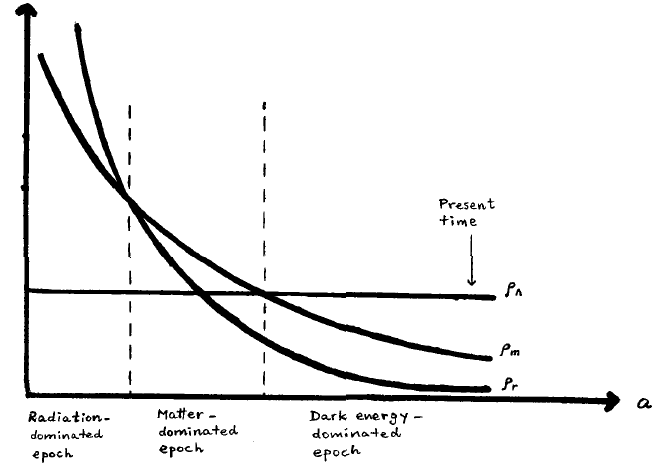
\includegraphics[scale=0.6]{Draw/lec6_2.png}
\end{center}
\caption{Evolution of the energy components of the universe}
\label{fig:lec6_2}
\end{figure}

\subsection{The universe with no dark energy}

We are now ready to study how the scale factor $a(t)$ changes in time. In this section we will consider a hypothetical universe with no dark energy, so we will set $\rho_{\Lambda}=0$. The Friedmann equation (\ref{eq:friedmann_eq}) then takes the form
\begin{equation} \label{eq:friedmann_eq1}
\left(\frac{\dot{a}}{a}\right)^2=\frac{8\pi G}{3c^2}\left( \frac{\rho_m(t_0)}{a^3}+\frac{\rho_r(t_0)}{a^4} \right)-\frac{kc^2}{R^2a^2}.
\end{equation}
Finding the exact solution of this equation is not easy, but we can get a qualitative understanding of how $a(t)$ evolves just by looking at the right-hand side of (\ref{eq:friedmann_eq1}). Consider first the cases where $k=0$ or $k=-1$. It is clear that, in these two cases, the right-hand side of the Friedmann equation is always positive, which implies that $\dot{a}(t)>0$ for all $t$. What this says is that the scale factor always increases in time, and so the universe will expand forever in the cases where $k=0$ or $k=-1$. This scenario is known as the Big Freeze (or the Big Chill), because the temperature of the universe will keep decreasing as the expansion continues.

Consider next the case $k=+1$. The curvature term is now negative (because of the negative sign), and so as $a$ increases this term will eventually become as large as the first term on the right-hand side of eq.\ (\ref{eq:friedmann_eq1}). At this time, then, we will have that $\dot{a}(t)=0$, which means that the expansion of the universe will stop. The universe will then begin to {\it contract}, and it will eventually recollapse in what is known as the Big Crunch (see fig.\ \ref{fig:lec6_3}).
\begin{figure}[ht]
\begin{center}
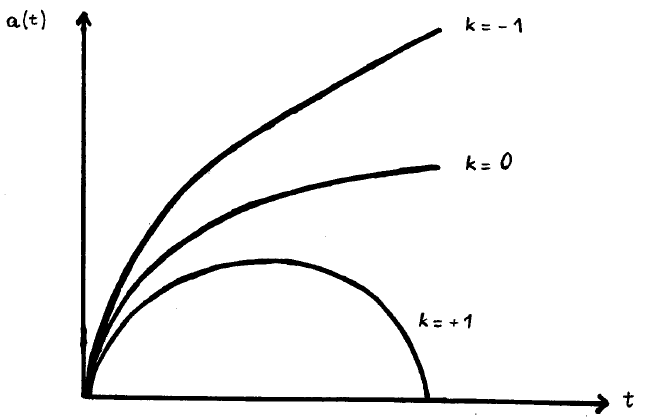
\includegraphics[scale=0.5]{Draw/lec6_3.png}
\end{center}
\caption{The universe with no dark energy}
\label{fig:lec6_3}
\end{figure}

\par\vspace{\baselineskip}

{\bf Exercise.} In the case $k=+1$, show that the value of $a$ at which $\dot{a}=0$ is given by
\begin{equation}
a=\frac{4\pi G}{3c^4}\frac{R^2}{k}\rho_m(t_0)\left[1+\sqrt{1+\frac{3c^4}{2\pi G}\frac{k}{R^2}\frac{\rho_r(t_0)}{\rho_m(t_0)^2}}\right].
\end{equation}

\par\vspace{\baselineskip}

We can then distinguish three types of universes depending on the spatial geometry and the evolution of the scale factor:
\begin{itemize}
\item Flat universe ($k=0$): The universe has zero spatial curvature, it is infinite in size, and it expands forever.
\item Open universe ($k=-1$): The universe has negative spatial curvature, it is infinite in size, and it expands forever.
\item Closed universe ($k=+1$): The universe has positive spatial curvature, it is finite in size, and it eventually recollapses.
\end{itemize}
Notice that the fact that the closed universe is finite in size does not mean that it has a boundary. If we start traveling in some direction we are not eventually going to find a wall at which the universe ends, but instead we are going to come back to the place where we started. This may seem odd for our ``Euclidean'' minds, which are not used to think in 3-dimensional curved spaces. However, the 2-dimensional analogy of the sphere is useful to understand this point. The space defined by the surface of a sphere is also a finite space with no boundaries; here if you walk in some direction (along the equator, for instance) you will eventually come back to the starting point. The same happens in the case of a closed universe, which has the spatial geometry of a 3-dimensional sphere.

\subsection{The universe with dark energy}

As we will see in a later lecture, today we have compelling evidence that there is dark energy in the universe. In fact, we will see below that dark energy is the dominant source of energy at the present time. If $\rho_{\Lambda}>0$ the Friedmann equation reads
\begin{equation} \label{eq:friedmann_eq2}
\left(\frac{\dot{a}}{a}\right)^2=\frac{8\pi G}{3c^2}\left( \frac{\rho_m(t_0)}{a^3}+\frac{\rho_r(t_0)}{a^4}+\rho_{\Lambda} \right)-\frac{kc^2}{R^2a^2}.
\end{equation}
There is no simple analytical solution to this equation. However, notice that the right-hand side of (\ref{eq:friedmann_eq2}) is always positive at late times, regardless of the value of $k$, thanks to the presence of the constant term proportional to $\rho_{\Lambda}$. This means that $\dot{a}(t)>0$ for large $t$, and so the scale factor will increase in time without bound. Thus, at late times we will have that $a\gg1$, implying that all the terms on the right-hand side of (\ref{eq:friedmann_eq2}) will be small, with the exception of the constant dark energy term, which is independent of $a$. In other words, the dark energy density will always dominate over the other energy sources (and over the curvature term) at sufficiently late times. Then, at late times, we can write the Friedmann equation in the approximate form
\begin{equation}
\left(\frac{\dot{a}}{a}\right)^2=\frac{8\pi G}{3c^2}\rho_{\Lambda},
\end{equation}
\begin{equation}
\Rightarrow~~~~\dot{a}=\sqrt{\frac{8\pi G}{3c^2}\rho_{\Lambda}}~a.
\end{equation}
If we take the time derivative of the last equation we obtain
\begin{equation}
\begin{split}
\ddot{a}&=\sqrt{\frac{8\pi G}{3c^2}\rho_{\Lambda}}~\dot{a}\\
&=\left(\frac{8\pi G}{3c^2}\rho_{\Lambda}\right) a,
\end{split}
\end{equation}
where $\ddot{a}(t)$ denotes the second time derivative of $a(t)$. The important conclusion is that $\ddot{a}(t)>0$ at late times. What this says is that the rate of expansion, $\dot{a}$, is itself increasing in time. In other words, the expansion of the universe is accelerating! The observation of this cosmic acceleration is one the most important discoveries of the past two decades, as it provided compelling evidence for the existence of dark energy (although other explanations exist, as we will see later). The qualitative evolution of the scale factor, in the presence of dark energy, is shown in fig.\ \ref{fig:lec6_4}. Notice that when $\rho_{\Lambda}>0$ the universe will expand forever in the future, regardless of the value of $k$, and regardless of whether the universe is finite or infinite in size.
\begin{figure}[ht]
\begin{center}
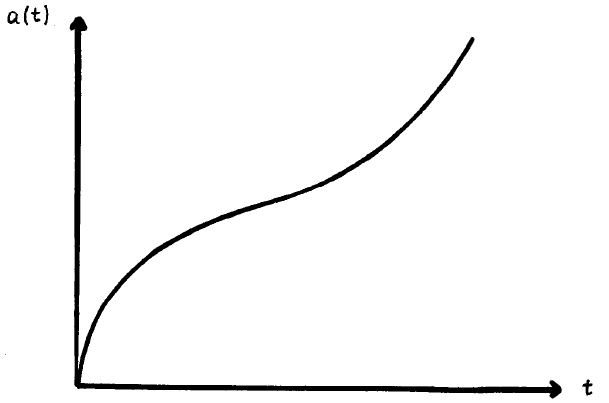
\includegraphics[scale=0.5]{Draw/lec6_4.png}
\end{center}
\caption{The universe with dark energy}
\label{fig:lec6_4}
\end{figure}

\subsection{Density parameters}

In this subsection we introduce the density parameters, which are useful tools used by cosmologists. First, recall the definition of the Hubble parameter,
\begin{equation}
H(t)\equiv \frac{\dot{a}(t)}{a(t)}.
\end{equation}
Recall also that the Hubble constant is simply the present value of the Hubble parameter: $H_0\equiv H(t_0)$, where $t_0$ denotes the present time. We can then write the Friedmann equation (\ref{eq:friedmann_eq}) in terms of $H(t)$ as follows:
\begin{equation}
H(t)^2= \frac{8\pi G}{3c^2}\rho(t)-\frac{kc^2}{R^2a(t)^2}.
\end{equation}
Dividing this equation by $H(t)^2$ we get
\begin{equation} \label{eq:friedmann_eq3}
1= \frac{8\pi G}{3c^2H(t)^2}\rho(t)-\frac{kc^2}{R^2H(t)^2a(t)^2}.
\end{equation}
Next define the {\it critical density} as
\begin{equation} \label{eq:crit_dens}
\rho_c(t)\equiv \frac{3c^2H(t)^2}{8\pi G}.
\end{equation}
The present value of $\rho_c$ (divided by $c^2$ to get a mass density) is given by
\begin{equation}
\begin{split}
\frac{\rho_c(t_0)}{c^2}&=\frac{3H_0^2}{8\pi G}\\
&\approx 10^{-26}~\mathrm{kg~m^{-3}}\approx 10^{11}~M_{\odot}~\mathrm{Mpc^{-3}},
\end{split}
\end{equation}
where $M_{\odot}$ denotes the solar mass. Using definition (\ref{eq:crit_dens}) in eq.\ (\ref{eq:friedmann_eq3}) we find
\begin{equation} \label{eq:friedmann_eq4}
1=\frac{\rho(t)}{\rho_c(t)}-\frac{kc^2}{R^2H(t)^2a(t)^2}.
\end{equation}
Finally, define the {\it density parameter} $\Omega(t)$ as
\begin{equation}
\Omega(t)\equiv \frac{\rho(t)}{\rho_c(t)}.
\end{equation}
Eq.\ (\ref{eq:friedmann_eq4}) can then be rewritten as
\begin{equation}
\Omega(t)-1=\frac{kc^2}{R^2H(t)^2a(t)^2}.
\end{equation}
Evaluating this last equation at $t=t_0$ (the present time), we find\footnote{Recall that $a(t_0)=1$ by definition.}
\begin{equation}
\Omega(t_0)-1=\frac{kc^2}{R^2H_0^2},
\end{equation}
\begin{equation} \label{eq:curvature_dens_param}
\Rightarrow~~~~\frac{k}{R^2}=\frac{H_0^2}{c^2}\left(\Omega(t_0)-1\right).
\end{equation}
Eq.\ (\ref{eq:curvature_dens_param}) is very useful, because it allows us to find the values of $k$ and $R$ if we know the values of $H_0$ and $\Omega(t_0)$, which can be directly measured. However, observations tell us that $\Omega(t_0)\approx1$, which implies that the right-hand side of eq.\ (\ref{eq:curvature_dens_param}) is approximately (if not exactly) zero. Therefore the left-hand side must also be zero or very close to zero. This means that either $k=0$ (and the universe is flat), or $k\neq0$ but $R$ is very large. Unfortunately, then, we cannot tell experimentally whether the universe is finite or infinite in size; however, if it is finite (so that $k=1$), then it must be much larger than the observable universe (whose size is of the order of $c/H_0$). The reason why $\Omega(t_0)$ is so close to unity is an important puzzle in cosmology; the theory of inflation (which we will study in a later lecture) is widely believed to provide the correct solution to this question.

Let us define next the density parameters for the matter, the radiation, and the dark energy, as follows:
\begin{equation}
\begin{split}
\Omega_m(t)&\equiv \frac{\rho_m(t)}{\rho_c(t)},\\
\Omega_r(t)&\equiv \frac{\rho_r(t)}{\rho_c(t)},\\
\Omega_{\Lambda}(t)&\equiv \frac{\rho_{\Lambda}}{\rho_c(t)}.\\
\end{split}
\end{equation}
The total density parameter $\Omega(t)$ can then be written as
\begin{equation}
\begin{split}
\Omega(t)&= \frac{\rho(t)}{\rho_c(t)}\\
&=\frac{\rho_m(t)}{\rho_c(t)}+\frac{\rho_r(t)}{\rho_c(t)}+\frac{\rho_{\Lambda}(t)}{\rho_c(t)},
\end{split}
\end{equation}
\begin{equation}
\Rightarrow~~~~\Omega(t)=\Omega_m(t)+\Omega_r(t)+\Omega_{\Lambda}(t).
\end{equation}
Let us look at the different energy components of the universe more closely. The matter in the universe includes the following:
\begin{itemize}
\item Baryonic matter (protons, neutrons, electrons)
\item Dark matter
\end{itemize}
We can accordingly write the matter density parameter as the sum of the baryonic density parameter, $\Omega_b(t)$, and the dark matter density parameter, $\Omega_{DM}(t)$. Thus,
\begin{equation}
\Omega_m(t)=\Omega_b(t)+\Omega_{DM}(t).
\end{equation}
Do not confuse dark matter with dark energy. Whereas dark energy is a form of energy whose nature is unknown, dark matter is really just another form of matter, meaning that it is composed of particles (there are however alternative theories, as we will see later in the course). The problem is that physicists do not know what kind of particle it is. We know that dark matter exists because of the gravitational force it exerts on stars and galaxies, but it is not known whether it interacts via any of the other forces. In particular, dark matter does not interact via the electromagnetic force, meaning that it cannot emit or absorb light (hence the name ``dark'').

The radiation in the universe includes all relativistic particle species, which at the present time are given by the following:
\begin{itemize}
\item Photons
\item Neutrinos
\end{itemize}
Photons are massless particles, and so they move at the speed of light and are therefore always relativistic. Neutrinos, on the other hand, are particles with very small, but nonzero masses. In the context of cosmology, the question of whether a massive particle is relativistic or not depends on its temperature. If the temperature is large, such that the thermal energy of a given particle (which is a measure of the mean kinetic energy) is larger than the rest energy, then the particle will be relativistic. If, on the other hand, the rest energy is much larger than the thermal energy (as occurs to baryons today), then the particle will be nonrelativistic. Since we do not know the precise values of the neutrino masses (and therefore we do not know the rest energy of a neutrino), we cannot actually be sure that neutrinos are relativistic today. However, we do know that neutrinos have been relativistic for most of the history of the universe, so that their relative importance in cosmology is similar to that of 
photons. This is why we will usually study neutrinos as being part of the radiation component of the energy in the universe.

With this in mind, we can write the radiation density parameter as the sum of the photon density parameter, $\Omega_{\gamma}(t)$, and the neutrino density parameter, $\Omega_{\nu}(t)$. Thus,
\begin{equation}
\Omega_r(t)=\Omega_{\gamma}(t)+\Omega_{\nu}(t).
\end{equation}

Finally, we can write the present density parameter $\Omega(t_0)$ in terms of all the different energy components present in the universe:
\begin{equation}
\Omega(t_0)=\Omega_b(t_0)+\Omega_{DM}(t_0)+\Omega_{\gamma}(t_0)+\Omega_{\nu}(t_0)+\Omega_{\Lambda}(t_0).
\end{equation}
Experimentally, these are given by
\begin{equation}
\begin{split}
\Omega_{\gamma}(t_0)&\approx 5\times10^{-5},\\
\Omega_{\nu}(t_0)&\approx 3\times10^{-5},\\
\Omega_{b}(t_0)&\approx 0.04,\\
\Omega_{DM}(t_0)&\approx 0.26,\\
\Omega_{\Lambda}(t_0)&\approx 0.70.
\end{split}
\end{equation}
As we mentioned above, the energy density today is dominated by the dark energy, which is about $70\%$ of the total energy. It is followed by the matter energy density, which today is about $30\%$ of the total energy. Finally, the radiation presently contributes only a small fraction to the energy density in the universe (see fig.\ \ref{fig:lec6_2}). Notice the (embarrasing) fact that $96\%$ of the energy density in the universe is in the form of dark matter and dark energy, whose exact nature is unknown.

\section{Aside on particle physics}

In this section we will make a quick introduction to particle physics. This will be useful for our study of the thermal history of the universe during this and next lectures.

There are four types of interactions (or forces) in nature: electromagnetic, weak, strong, and gravitational. Each interaction is mediated by one or more particles called {\it bosons}.\footnote{More precisely, the particles that mediate the interactions are called gauge bosons. A different type of boson is the Higgs, whose role is to give mass to all the other particles.} These are shown in the following table:
\begin{table}[ht]
\begin{center}
\begin{tabular}{p{4cm} l l} \hline\hline
Interaction & Boson  \\ \hline
Electromagnetic & Photon \\
Weak & $W^{+}$, $W^{-}$, $Z^0$ \\
Strong & Gluon \\
Gravitational & Graviton \\ \hline\hline
\end{tabular}
\end{center}
\end{table}

The particles that form matter (including antimatter and unstable matter) are called {\it fermions}. Fermions are divided into {\it leptons} and {\it quarks}. Leptons are further divided into charged leptons and neutrinos. This classification is summarized in the following diagram:
\begin{equation*}
\mbox{Fermions }\begin{cases} \mbox{$~~$Leptons } \begin{cases} \mbox{$~~$Charged leptons}\\ ~\\ \mbox{$~~$Neutrinos}\end{cases}\\ 
~\\
\mbox{$~~$Quarks} \end{cases}
\end{equation*}
Each fermion has a corresponding antiparticle, which has the same mass but opposite quantum numbers. For example, if a particle has negative electric charge the antiparticle has a positive electric charge of the same magnitude. The different fermions presently known are described in the following:
\begin{itemize}
\item Charged leptons: electron ($e^{-}$), muon ($\mu^{-}$), tau ($\tau^{-}$) (antiparticles: $e^{+}$, $\mu^{+}$, $\tau^{+}$). They interact via the electromagnetic, the weak, and the gravitational forces.
\item Neutrinos: electron neutrino ($\nu_e$), muon neutrino ($\nu_{\mu}$), tau neutrino ($\nu_{\tau}$) (antiparticles: $\bar{\nu}_e$, $\bar{\nu}_{\mu}$, $\bar{\nu}_{\tau}$). They interact via the weak and the gravitational forces.
\item Quarks: up ($u$), down ($d$), strange ($s$), charm ($c$), bottom ($b$), top ($t$) (antiparticles: $\bar{u}$, $\bar{d}$, $\bar{s}$, $\bar{c}$, $\bar{b}$, $\bar{t}$). They interact via the electromagnetic, the weak, the strong, and the gravitational forces.
\end{itemize}
An important property of quarks is called {\it quark confinement}: at temperatures below $T\sim 2\times10^{12}$ K, quarks cannot be found as free particles, but are confined within composite particles known as {\it hadrons}.\footnote{Compare the quark confinement temperature with the temperature at the core of the Sun: $1.6\times10^7$ K.} There are two types of hadrons: {\it baryons} (particles formed by 3 quarks), and {\it mesons} (particles formed by 2 quarks). Examples of baryons include the familiar proton and neutron.\footnote{An important note on terminology: In astrophysics and cosmology people often refer to protons, neutrons and electrons as ``baryons,'' although electrons are not really baryons in the classification of particle physics.} Examples of mesons include the pion and the kaon.
\begin{equation*}
\mbox{Hadrons }\begin{cases} \mbox{$~~$Baryons} \\ 
~\\
\mbox{$~~$Mesons} \end{cases}
\end{equation*}

The picture we have just decribed is known as the Standard Model of particle physics, and it is one of the most successful theories in the history of physics (fig.\ \ref{fig:lec6_5}).\footnote{Actually, the graviton has not been detected yet, and it is not part of the Standard Model} We know, however, that this picture has to be incomplete: it does not include dark matter. Dark matter interacts only via the gravitational force, and perhaps via the weak force. The only candidate with these properties, within the Standard Model, is the neutrino. However, we will see later that, because of their very small mass, neutrinos cannot be the dark matter, which means that we have to look at other theories that include new (and so far unobserved) particles for possible dark matter candidates.
\begin{figure}[ht]
\begin{center}
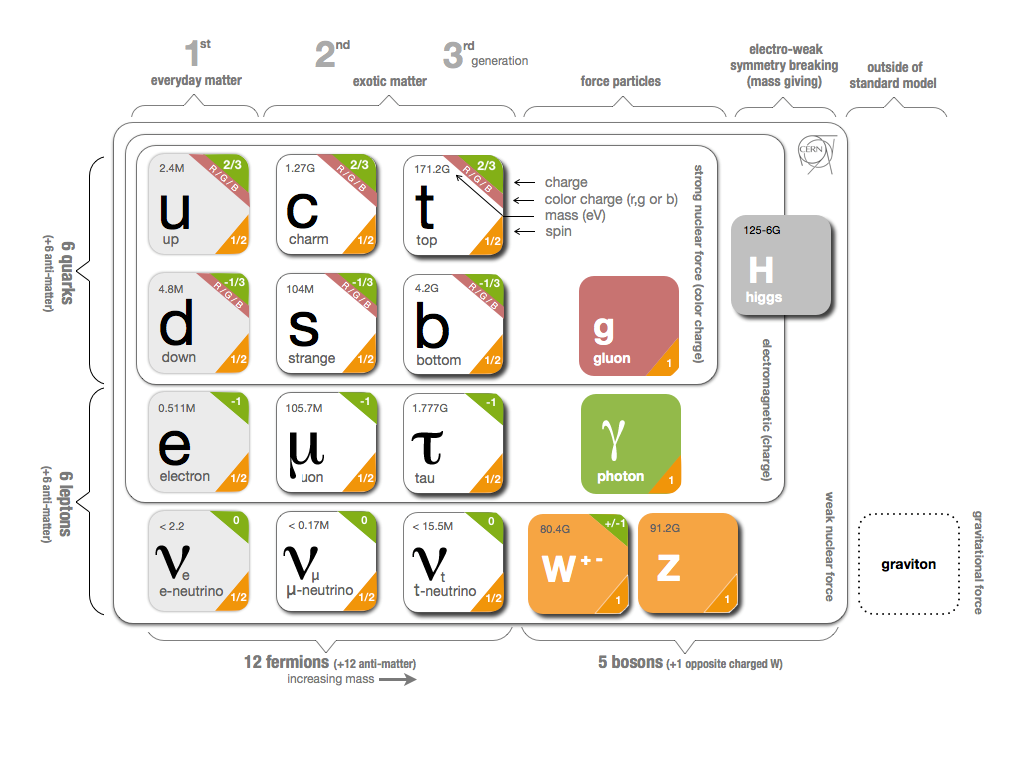
\includegraphics[scale=0.35]{Draw/lec6_5.png}
\end{center}
\caption{The particles of the Standard Model (Source: \url{http://www.isgtw.org})}
\label{fig:lec6_5}
\end{figure}

\section{The thermal history of the universe}
\label{chp7}

The early universe can be thought of as a soup (more technically a plasma) of {\it primordial particles} (particles created during the very first instants after the Big Bang) continuously interacting with each other in a state of thermal equilibrium. A fluid or plasma in thermal equilibrium can be described by its temperature $T$, which is a measure of the average kinetic energy of the particles. Immediately after the Big Bang the temperature of the cosmic plasma is infinitely high, and then begins to continuously decrease as the universe expands. In fact, we will see in a later lecture that $T\propto 1/a$ during most of the history of the universe.

The strength at which particles interact depends on their kinetic energy, and therefore on the temperature of the plasma. At very high temperatures, all interactions are effective and all particles are maintained in thermal equilibrium with the plasma. As the temperature decreases, however, some interactions become inefficient and some particle species may fall out of equilibrium with the plasma, in a process known as {\it decoupling}, and subsequently travel freely through the universe, without further scatterings with the other particles in the plasma. This is what happened to neutrinos when the universe was only $0.2$ seconds old, and later to photons when the universe was about $380,000$ years old.\footnote{There is also an earlier stage at which dark matter particles decoupled from the cosmic plasma. The details of this stage are largely unknown, and so we will omit it in the following outline.}

In what follows we will make a quick outline of the main phases of the thermal history of the universe, with the corresponding times and temperatures. In the following lectures we will cover some these phases in much more detail.

\begin{itemize}

\item $t\sim 10^{-5}$ s, $T\sim 2\times10^{12}$ K: Quark confinement.

By this time all the muons and tau leptons, as well as all the quarks heavier than the $u$ and $d$, have decayed. The cosmic plasma now contains electrons, neutrinos, $u$ quarks, $d$ quarks, and photons. After this time quarks become confined and form the first protons and neutrons.

\item $t\sim 0.2$ s, $T\sim 10^{10}$ K: Neutrino decoupling.

Neutrinos interact with the other particles in the plasma only via the weak force (and also via the gravitational force, but this is completely negligible). This is what keeps the neutrinos in thermal equilibrium with the plasma. However, when the temperature drops below $T\sim 10^{10}$ K, the weak interaction becomes inefficient. Neutrinos then decouple from the plasma and begin to propagate freely without further interactions.

\item $t\sim 200$ s, $T\sim 5\times10^8$ K: Nucleosynthesis.

At temperatures above $T\sim 5\times10^8$ K protons and neutrons are free; they cannot bind together to form heavier atomic nuclei (such as helium), since the photons in the plasma immediately destroy them. This effect is known as {\it nuclear photodissociation}. When the temperature drops below $T\sim 5\times10^8$ K the photons are not energetic enough to destroy the nuclei effectively, and protons and neutrons can now combine to form the first atomic nuclei: deuterium ($^2$H), tritium ($^3$H), helium-3 ($^3$He), helium-4 ($^4$He), and lithium ($^7$Li). This process is known as {\it nucleosynthesis}.

\item $t\sim 10^{13}$ s, $T\sim 4\times10^3$ K: Recombination.

By this time the cosmic plasma contains electrons, photons, and atomic nuclei. At temperatures above $T\sim 4\times10^3$ K there are no neutral atoms; as soon as an electron is captured by a nucleus to form a neutral atom, it is immediately kicked out by a photon in a process known as {\it photoionization}. When the temperature drops below $T\sim 4\times10^3$ K the photons in the plasma are not energetic enough to ionize the atoms effectively. As a result, electrons quickly become captured by atomic nuclei and the universe becomes neutral: it now contains only atoms, photons, neutrinos, and dark matter. This process is known as {\it recombination}. Since photons can only interact with electrically charged particles, after recombination the primordial photons decouple and begin to propagate without further interactions. These are the photons that we can observe today in the cosmic microwave background (CMB).

\item $t\sim 10^{16}-10^{17}$ s: Structure formation.

After recombination the cosmic plasma disappears. The remaining neutral atoms (as well as the dark matter) begin to clump together as a result of gravity. Eventually the lumps of atoms grow larger and larger until they form the first stars and galaxies. This is the process of {\it structure formation}, which includes several stages whose exact details are not yet fully understood.

\end{itemize}